\documentclass{beamer}
\usepackage{tikz,amsmath,hyperref,graphicx,stackrel,animate}
\usetikzlibrary{positioning,shadows,arrows,shapes,calc,dsp,chains}
\newcommand{\argmax}{\operatornamewithlimits{argmax}}
\newcommand{\argmin}{\operatornamewithlimits{argmin}}
\mode<presentation>{\usetheme{Frankfurt}}
\AtBeginSection[]
{
  \begin{frame}<beamer>
    \frametitle{Outline}
    \tableofcontents[currentsection,currentsubsection]
  \end{frame}
}
\title{Lecture 14: Notch Filters}
\author{Mark Hasegawa-Johnson}
\date{ECE 401: Signal and Image Analysis, Fall 2020}  
\begin{document}

% Title
\begin{frame}
  \maketitle
\end{frame}

% Title
\begin{frame}
  \tableofcontents
\end{frame}

%%%%%%%%%%%%%%%%%%%%%%%%%%%%%%%%%%%%%%%%%%%%
\section[Review]{Review: Poles and Zeros}
\setcounter{subsection}{1}

\begin{frame}
  \frametitle{Review: Poles and Zeros}
  A first-order autoregressive filter,
  \[
  y[n] = x[n]+bx[n-1]+ay[n-1],
  \]
  has the impulse response and transfer function
  \[
  h[n]=a^n u[n]+ba^{n-1}u[n-1] \leftrightarrow H(z)  = \frac{1+bz^{-1}}{1-az^{-1}},
  \]
  where $a$ is called the {\bf pole} of the filter, and $-b$ is called
  its {\bf zero}.
\end{frame}

\begin{frame}
  \frametitle{Review: Poles and Zeros}

  Suppose $H(z)=\frac{1+bz^{-1}}{1-az^{-1}}$.  Now let's evaluate
  $|H(\omega)|$, by evaluating $|H(z)|$ at $z=e^{j\omega}$:
  \[
  \vert H(\omega)\vert = 
  \frac{\vert e^{j\omega}+b\vert}{\vert e^{j\omega}-a\vert}
  \]
  What it means $|H(\omega)|$ is the ratio of two vector lengths:
  \begin{itemize}
  \item When the vector length $|e^{j\omega}+b|$ is small, then
    $|H(\omega)|$ is small.
  \item When $|e^{j\omega}-a|$ is small, then $|H(\omega)|$ is LARGE.
  \end{itemize}
\end{frame}

\begin{frame}
  \frametitle{Review: Parallel Combination}

  Parallel combination of two systems looks like this:
  \vspace*{3mm}

  \centerline{\begin{tikzpicture}
      \node[dspnodeopen,dsp/label=right] (y) at (2,0) {$y[n]$};
      \node[dspadder] (adder) at (1,0) {}  edge[dspflow] (y);
      \node[coordinate] (y1) at (1,1) {}  edge[dspline] (adder);
      \node[coordinate] (y2) at (1,-1) {}  edge[dspline] (adder);
      \node[dspsquare] (h1) at (0,1) {$H_1(z)$}  edge[dspline] (y1);
      \node[dspsquare] (h2) at (0,-1) {$H_2(z)$}  edge[dspline] (y2);
      \node[coordinate] (x1) at (-1,1) {}  edge[dspconn] (h1);
      \node[coordinate] (x2) at (-1,-1) {}  edge[dspconn] (h2);
      \node[dspnodefull] (xsplit) at (-1,0) {} edge[dspline](x1) edge[dspline](x2);
      \node[dspnodeopen,dsp/label=left] (x) at (-2,0) {$x[n]$} edge[dspline] (xsplit);
  \end{tikzpicture}}
  Suppose that we know each of the systems separately:
  \[
  H_1(z)=\frac{1}{1-p_1z^{-1}},~~~~~
  H_2(z)=\frac{1}{1-p_2z^{-1}}
  \]
  Then, to get $H(z)$, we just  have to add:
  \[
  H(z) = \frac{1}{1-p_1z^{-1}}+\frac{1}{1-p_2z^{-1}}
  \]
\end{frame}

\begin{frame}
  \frametitle{Review: Parallel Combination}

  Parallel combination of two systems looks like this:
  \vspace*{3mm}

  \centerline{\begin{tikzpicture}
      \node[dspnodeopen,dsp/label=above] (y) at (2,0) {$y[n]$};
      \node[dspadder] (adder) at (1,0) {}  edge[dspflow] (y);
      \node[coordinate] (y1) at (1,1) {}  edge[dspline] (adder);
      \node[coordinate] (y2) at (1,-1) {}  edge[dspline] (adder);
      \node[dspsquare] (h1) at (0,1) {$H_1(z)$}  edge[dspline] (y1);
      \node[dspsquare] (h2) at (0,-1) {$H_2(z)$}  edge[dspline] (y2);
      \node[coordinate] (x1) at (-1,1) {}  edge[dspconn] (h1);
      \node[coordinate] (x2) at (-1,-1) {}  edge[dspconn] (h2);
      \node[dspnodefull] (xsplit) at (-1,0) {} edge[dspline](x1) edge[dspline](x2);
      \node[dspnodeopen,dsp/label=above] (x) at (-2,0) {$x[n]$} edge[dspline](xsplit);
  \end{tikzpicture}}
  \begin{align*}
  H(z) &= \frac{1}{1-p_1z^{-1}}+\frac{1}{1-p_2z^{-1}}\\
  &= \frac{1-p_2z^{-1}}{(1-p_1z^{-1})(1-p_2z^{-1})}+\frac{1-p_1z^{-1}}{(1-p_1z^{-1})(1-p_2z^{-1})}\\
  &= \frac{2-(p_1+p_2)z^{-1}}{1-(p_1+p_2)z^{-1}+p_1p_2z^{-2}}
  \end{align*}
\end{frame}

\begin{frame}
  \frametitle{Review: Complex Numbers}

  Suppose that
  \begin{align*}
    p_1 &= x_1+jy_1 = |p_1|e^{j\theta_1}\\
    p_2=p_1^* &= x_1-jy_1 = |p_1|e^{-j\theta_1}
  \end{align*}
  Then
  \begin{itemize}
  \item $p_1+p_2$ is real:
    \begin{displaymath}
      p_1+p_2 = x_1+jy_1 + x_1-jy_1 = 2x_1
    \end{displaymath}
  \item $p_1p_2$ is also real:
    \begin{displaymath}
      p_1p_2 = |p_1|e^{j\theta_1} |p_1|e^{-j\theta_1} = |p_1|^2
    \end{displaymath}
  \end{itemize}
\end{frame}

%%%%%%%%%%%%%%%%%%%%%%%%%%%%%%%%%%%%%%%%%%%%
\section[Line Noise]{Using Zeros to Cancel Line Noise}
\setcounter{subsection}{1}

\begin{frame}
  \frametitle{The problem of electrical noise}

  When your microphone cable is too close to an electrical cord, you
  often get noise at the harmonics of 60Hz (especially at 120Hz as
  shown here; sometimes also at 180Hz and 240Hz).
  \centerline{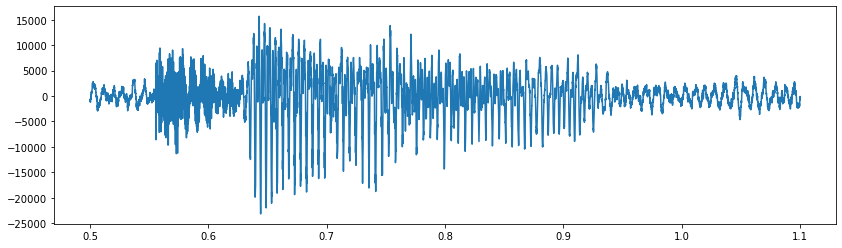
\includegraphics[width=4.5in]{waveform_with_120hz.png}}
\end{frame}

\begin{frame}
  \frametitle{Can we use zeros?}

  As you know, zeros in $H(z)$ cause dips in $H(\omega)$.  Can we use that, somehow,
  to cancel out noise at a particular frequency?
  \centerline{\animategraphics[loop,controls,width=4.5in]{10}{../lec11/exp/magresponse}{0}{99}}
\end{frame}

\begin{frame}
  \frametitle{Can we use zeros?}

  In particular,
  \[
  H(z)  = \frac{1+bz^{-1}}{1-az^{-1}}
  \]
  \begin{itemize}
  \item The pole needs to have a magnitude less than one ($|a|<1$),
    otherwise the filter will be unstable, but\ldots
  \item the zero doesn't have that restriction.  We can set $|b|=1$ if we want to.
  \item In particular, suppose we want to completely cancel all inputs
    at $\omega=\omega_c$.  Can we just set $H(e^{j\omega_c})=0$?
  \end{itemize}
\end{frame}

\begin{frame}
  \frametitle{{\bf Q}: Can we just set $H(e^{j\omega_c})=0$?\\{\bf A: YES!}}
  \centerline{\animategraphics[loop,controls,width=4.5in]{10}{exp/onezeroresponse}{0}{49}}
\end{frame}  

\begin{frame}
  \frametitle{Using Zeros to Cancel Line Noise}
  The filter shown in the previous slide is just $H(z)=1+bz^{-1}$, i.e.,
  \begin{displaymath}
    y[n] = x[n] + bx[n-1]
  \end{displaymath}
  There are two problems with this filter:
  \begin{enumerate}
  \item {\bf Complex:} $b$ needs to be complex, therefore $y[n]$ will
    be complex-valued, even if $x[n]$ is real.  Can we design a filter
    with a zero at $z=-b$, but with real-valued outputs?
  \item {\bf Distortion:} $H(z)$ cancels the line noise, but it also
    changes signal amplitudes at every other frequency.
  \end{enumerate}
\end{frame}

\begin{frame}
  \frametitle{Complex Conjugate Zeros}

  The problem of complex outputs is solved by choosing
  complex-conjugate zeros.  Suppose we choose zeros at
  \begin{displaymath}
    r_1 = e^{j\omega_c},~~~r_2=r_1^*=e^{-j\omega_c}
  \end{displaymath}
  Then the filter is
  \begin{displaymath}
    H(z) = (1-r_1z^{-1})(1-r_2z^{-1}) = 1-(r_1+r_2)z^{-1} + r_1r_2z^{-2},
  \end{displaymath}
  but from our review of complex numbers, we know that
  \begin{align*}
    r_1+r_2 &= 2\Re(r_1) = 2\cos(\omega_c)\\
    r_1r_2 &= |r_1|^2 = 1
  \end{align*}
\end{frame}

\begin{frame}
  \frametitle{Complex Conjugate Zeros}
  
  So the filter is 
  \begin{displaymath}
    H(z) = (1-r_1z^{-1})(1-r_2z^{-1}) = 1-2\cos(\omega_c) z^{-2} + z^{-2}.
  \end{displaymath}
  In other words,
  \begin{displaymath}
    y[n] = x[n] - 2\cos(\omega_c)x[n-1] + x[n-2]
  \end{displaymath}
  Its impulse response is
  \begin{displaymath}
    h[n]=\begin{cases}
    1 & n=0\\
    -2\cos\omega_c & n=1\\
    1 & n=2\\
    0 & \mbox{otherwise}
    \end{cases}
  \end{displaymath}
\end{frame}

\begin{frame}
  \frametitle{Complex Conjugate Zeros}
  \centerline{\animategraphics[loop,controls,width=4.5in]{10}{exp/twozeroresponse}{0}{49}}
\end{frame}  

%%%%%%%%%%%%%%%%%%%%%%%%%%%%%%%%%%%%%%%%%%%%
\section[Notch Filters]{Notch Filters}
\setcounter{subsection}{1}

\begin{frame}
  \frametitle{Distortion}

  \begin{itemize}
    \item The two-zero filter cancels line noise, but it also distorts the
      signal at every other frequency.
    \item Specifically, it amplifies signals in proportion as their
      frequency is far away from $\omega_c$.  Since $\omega_c$ is probably
      low-frequency, $H(z)$ probably makes the signal sound brassy or tinny.
    \item Ideally, we'd like the following frequency response.  Is this possible?
      \begin{displaymath}
        H(\omega) = \begin{cases}
          0 & \omega=\omega_c \\
          1 & \mbox{most other frequencies}
        \end{cases}
      \end{displaymath}
  \end{itemize}
\end{frame}

\begin{frame}
  \frametitle{Notch Filter: A Pole for Every Zero}

  The basic idea of a notch filter is to have a pole for every zero.
  \begin{displaymath}
    H(z)=\frac{1-rz^{-1}}{1-pz^{-1}},~~~|H(\omega)|=\frac{|1-re^{-j\omega}|}{|1-pe^{-j\omega}|}
  \end{displaymath}
  and then choose $r=e^{j\omega_c}$ and $p=ae^{j\omega_c}$, for some
  $a$ that is very close to 1.0, but not quite 1.0.  That way,
  \begin{itemize}
  \item When $\omega=\omega_c$, the numerator is exactly
    \begin{displaymath}
      |1-e^{j(\omega_c-\omega_c)}|=|1-1|=0
    \end{displaymath}
  \item When $\omega\ne\omega_c$,
    \begin{displaymath}
      |e^{j\omega}-r|\approx |e^{j\omega}-p|,~~~\mbox{so}~~~|H(\omega)|\approx 1
    \end{displaymath}
  \end{itemize}
\end{frame}

\begin{frame}
  \frametitle{Notch Filter: A Pole for Every Zero} The red line is
  $|e^{j\omega}-r|$ (distance to the zero on the unit circle).  The
  blue line is $|e^{j\omega}-p|$ (distance to the pole inside the unit
  circle).  They are almost the same length.
  \centerline{\animategraphics[loop,controls,width=4.5in]{10}{exp/onezeronotch}{0}{49}}
\end{frame}

\begin{frame}
  \frametitle{Notch Filter: Practical Considerations}

  Now let's consider two practical issues:
  \begin{itemize}
  \item How do you set the bandwidth of the notch?
  \item How do you get real-valued coefficients in the difference equation?
  \end{itemize}
\end{frame}

\begin{frame}
  \frametitle{Bandwidth of the Notch}

  In signal processing, we often talk about the ``3dB Bandwidth'' of a
  zero, pole, or notch.  Decibels (dB)  are defined as
  \begin{displaymath}
    \mbox{Decibels} = 20\log_{10}|H(\omega)| = 10\log_{10}|H(\omega)|^2
  \end{displaymath}
  The 3dB bandwidth of a notch is the bandwidth, $B$, at which
  $20\log_{10}|H\left(\omega_c\pm \frac{B}{2}\right)|=-3$dB.  This is a convenient number because
  \begin{displaymath}
    -3 \approx 20\log_{10}\left(\frac{1}{\sqrt{2}}\right),
  \end{displaymath}
  so when we talk about 3dB bandwidth, we're really talking about the
  bandwidth at which $|H(\omega)|$ is $\frac{1}{\sqrt{2}}$.
\end{frame}

\begin{frame}
  \frametitle{Bandwidth of the Notch}

  The 3dB bandwidth of a notch filter is the frequency
  $\omega=\omega_c+\frac{B}{2}$ at which
  \begin{displaymath}
    \frac{1}{\sqrt{2}} = \frac{|1-rz^{-1}|}{|1-pz^{-1}|}
  \end{displaymath}
  Let's plug in $z=e^{j(\omega_c+B/2)}$, $r=e^{j\omega_c}$, and $p=ae^{j\omega_c}$, we get
  \begin{displaymath}
    \frac{1}{\sqrt{2}} = \frac{|1-e^{j(\omega-\omega_c)}|}{|1-ae^{j(\omega-\omega_c)}|}
    = \frac{|1-e^{jB/2}|}{|1-ae^{jB/2}|}
    = \frac{|1-e^{jB/2}|}{|1-e^{\ln(a)+jB/2}|}.
  \end{displaymath}
  Let's use the approximation $e^x\approx 1+x$, and then 
  solve for $B$.  We get:
  \begin{displaymath}
    \frac{1}{\sqrt{2}}=\frac{|-jB/2|}{|-\ln(a)-jB/2|}
    ~~~\Rightarrow~~~B = - 2\ln(a)
  \end{displaymath}
\end{frame}

\begin{frame}
  \frametitle{Bandwidth $B= -2\ln(a)$}

  \centerline{\includegraphics[width=4.5in]{exp/notch100bw.png}}
\end{frame}
\begin{frame}
  \frametitle{Bandwidth $B= -2\ln(a)$}

  \centerline{\includegraphics[width=4.5in]{exp/notch20bw.png}}
\end{frame}

\begin{frame}
  \frametitle{First-Order Notch Filter has Complex Outputs}

  A notch filter is
  \begin{displaymath}
    H(z)=\frac{1-rz^{-1}}{1-pz^{-1}}
  \end{displaymath}
  which we implement using just one line  of python:
  \begin{displaymath}
    y[n] = x[n]-rx[n-1]+py[n-1]
  \end{displaymath}
  The problem: $r$ and $p$ are both complex, therefore, even if $x[n]$ is real,
  $y[n]$ will be complex.
\end{frame}

\begin{frame}
  \frametitle{Real-Valued Coefficients $\Leftrightarrow$ Conjugate Zeros and Poles}

  To get real-valued coefficients, we have to use a second-order
  filter with complex conjugate poles and zeros
  ($r_2=r_1^*=e^{-j\omega_c}$ and $p_2=p_1^*=ae^{-j\omega_c}$):
  \begin{align*}
    H(z)&=\frac{(1-r_1z^{-1})(1-r_1^*z^{-1})}{(1-p_1z^{-1})(1-p_1^*z^{-1})}\\
    &=\frac{1-(r_1+r_1^*)z^{-1}+|r_1|^2z^{-2}}{1-(p_1+p_1^*)z^{-1}+|p_1|^2 z^{-2}}\\
    &=\frac{1-2\cos\omega_c z^{-1}+ z^{-2}}{1-2a\cos\omega_c z^{-1}+a^2 z^{-2}}
  \end{align*}
  So then, we can implement it as a second-order difference equation, using just one line
  of code in python:
  \begin{displaymath}
    y[n]=x[n]-2\cos\omega_cx[n-1]+x[n-2]+2a\cos\omega_cy[n-1]-a^2y[n-2]
  \end{displaymath}
\end{frame}
\begin{frame}
  \frametitle{Real-Valued Coefficients $\Leftrightarrow$ Conjugate Zeros and Poles}
  If the poles and zeros come in conjugate pairs, then we get
  \begin{displaymath}
    H(z)=\frac{(1-r_1z^{-1})(1-r_1^*z^{-1})}{(1-p_1z^{-1})(1-p_1^*z^{-1})}
    =\frac{b_0+b_1z^{-1}+b_2z^{-2}}{1-a_1z^{-1}-a_2z^{-2}}
  \end{displaymath}
  where all the coefficients are real-valued:
  \begin{align*}
    b_0 &= 1\\
    b_1 &= -2\cos\omega_c\\
    b_2 &= 1\\
    a_1 &= 2a\cos\omega_c\\
    a_2 &= -a^2
  \end{align*}
\end{frame}

\begin{frame}
  \frametitle{Notch Filter with Conjugate-Pair Zeros and Poles}
  \begin{displaymath}
    |H(\omega)|=\frac{|e^{j\omega}-r_1|\times|e^{j\omega}-r_2|}{|e^{j\omega}-p_1|\times|e^{j\omega}-p_2|}
  \end{displaymath}
  \centerline{\animategraphics[loop,controls,width=4.5in]{10}{exp/twozeronotch}{0}{49}}
\end{frame}

\begin{frame}
  \frametitle{Summary: How to Implement a Notch Filter}

  To implement a notch filter at frequency $\omega_c$ radians/sample,
  with a bandwidth of $-\ln(a)$ radians/sample, you implement the difference equation:
  \begin{displaymath}
    y[n] = x[n]-2\cos(\omega_c)x[n-1]+x[n-2]-2a\cos(\omega_c)y[n-1]+a^2y[n-2]
  \end{displaymath}
  which gives you the notch filter
  \begin{displaymath}
    H(z) = \frac{(1-r_1z^{-1})(1-r_1^*z^{-1})}{(1-p_1z^{-1})(1-p_1^*z^{-1})}
  \end{displaymath}
\end{frame}

%%%%%%%%%%%%%%%%%%%%%%%%%%%%%%%%%%%%%%%%%%%%
\section[Summary]{Summary}
\setcounter{subsection}{1}
  
\begin{frame}
  \frametitle{Summary: How to Implement a Notch Filter}

  To implement a notch filter at frequency $\omega_c$ radians/sample,
  with a bandwidth of $-\ln(a)$ radians/sample, you implement the difference equation:
  \begin{displaymath}
    y[n] = x[n]-2\cos(\omega_c)x[n-1]+x[n-2]-2a\cos(\omega_c)y[n-1]+a^2y[n-2]
  \end{displaymath}
  which gives you the notch filter
  \begin{displaymath}
    H(z) = \frac{(1-r_1z^{-1})(1-r_1^*z^{-1})}{(1-p_1z^{-1})(1-p_1^*z^{-1})}
  \end{displaymath}
  with the magnitude response:
  \begin{displaymath}
    |H(\omega)| =\begin{cases}
    0 & \omega_c\\
    \frac{1}{\sqrt{2}} & \omega_c \pm \ln(a)\\
    \approx 1 & omega < \omega+\ln(a)~\mbox{or}~\omega > \omega-\ln(a)
    \end{cases}
  \end{displaymath}
\end{frame}

\end{document}
